\subsection{Implementation}
\begin{figure}[H]
    \centering
    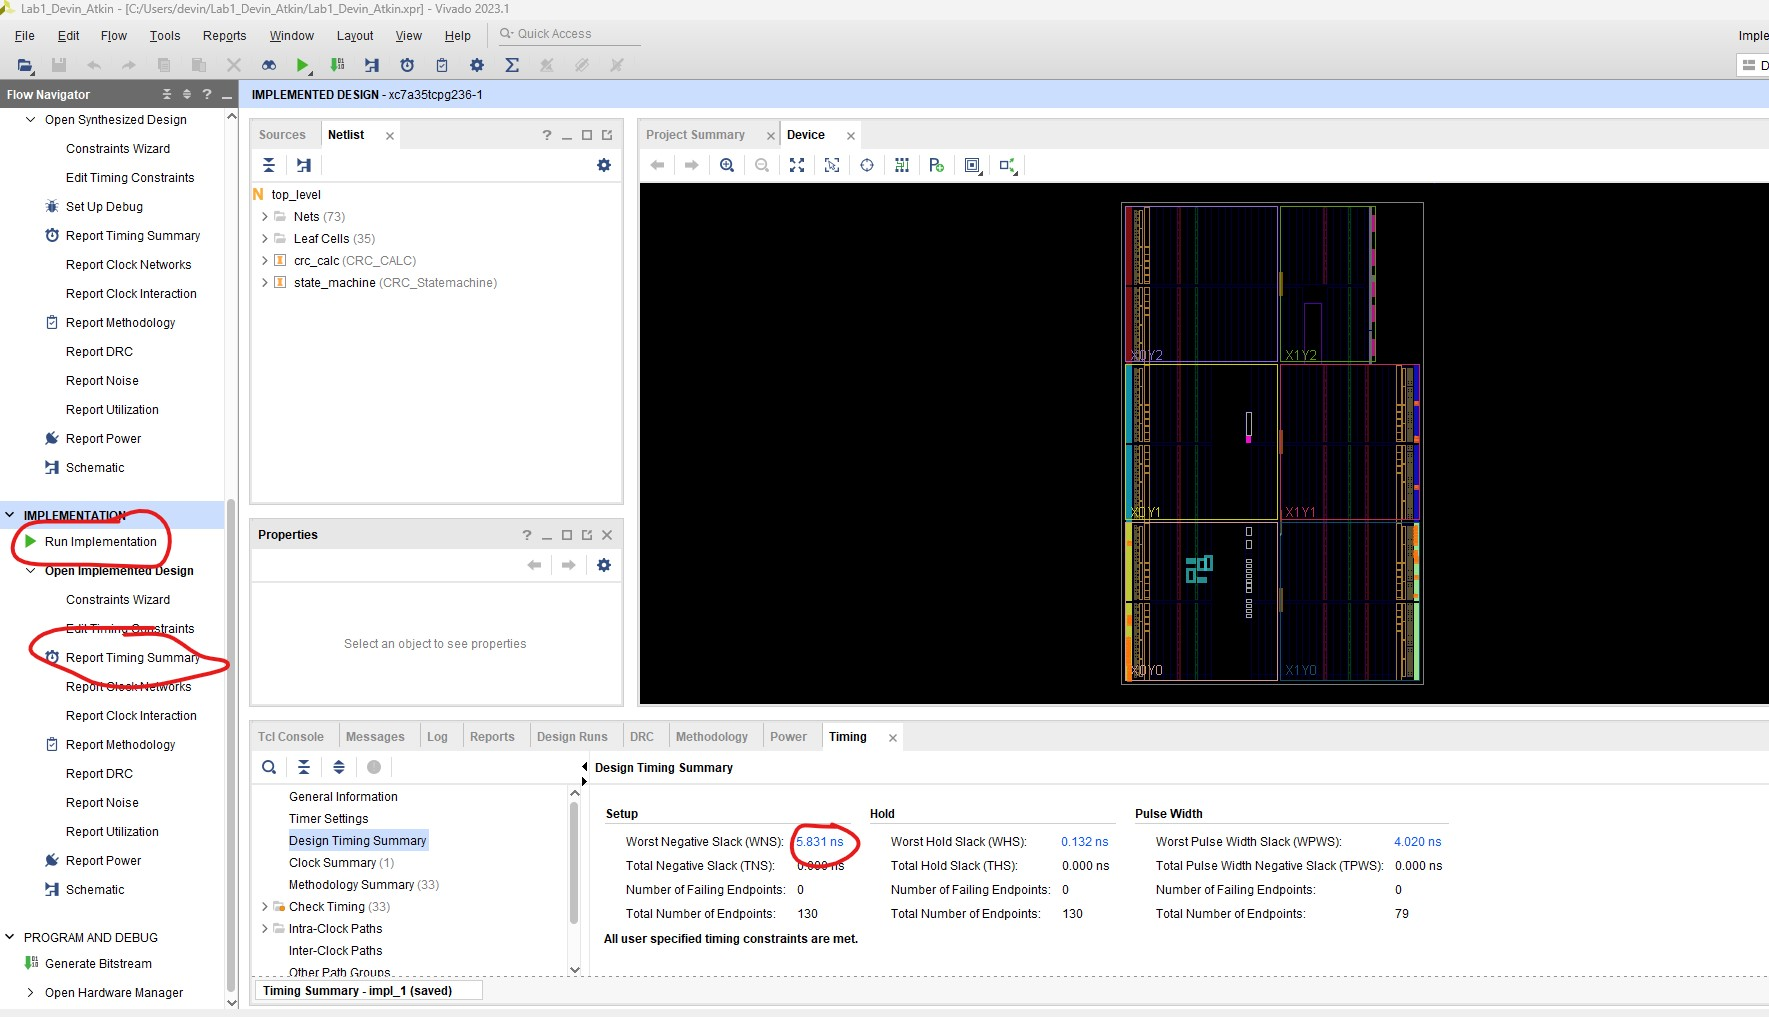
\includegraphics[width=9cm]{Images/CreateProjectImages/Implementation.jpg}
    \caption{Make sure to include your timing summary}
    \label{fig:enter-label}
\end{figure}
You will need to include the timing details on your lab design reports. You get this from the implementation. The timing summary should come up after implemention is run assuming you open the implemented design; however, if it doesn't you can get the timing summary by clicking \textit{Report Timing Summary} and then clicking ok for the default report. To Note, there is a separate timing report at the synthesis level which you don't necessarily need to pay attention to; however, if it fails to pass, implementation will almost definitely also fail to pass as well. 

\vspace{1cm}
\textbf{All of your designs must pass timing}. This means that they must be able to run at at least the 100MHz built in clock used by the Basys3. You are unlikely to run into timing issues on labs 1 and 2; however, this may become a challenge on labs 3 and 4 if you aren't careful when it comes to doing math. 

\vspace{0.5cm}
Use the following equation to calculate the maximum operating frequency for your design.
\[f_{max} = \frac{1}{t_{per}-t_{wns}} \]
Where \(f_{max}\) is the maximum operating frequency, \(t_{per}\) is the target period (in this case 10ns), and \(t_{wns}\) is the worst negative slack for the given implementation. The target period is determined by the clock speed of the design, this is defined in the constraints file for the project. You can see the clock being created here:

\begin{small}
\begin{verbatim}
## Clock signal
set_property PACKAGE_PIN W5 [get_ports CLK]							
set_property IOSTANDARD LVCMOS33 [get_ports CLK]
create_clock -add -name sys_clk_pin -period 10.00 -waveform {0 5} [get_ports CLK]
\end{verbatim}
\end{small}
The period is after the -period and is expressed in nanoseconds. However, this is determined by the crystal oscillator on the Basys3. If we were performing logic which required a slower clock speed, we would have to use either clock dividers or a PLL on chip to generate the alternate frequency. 